\documentclass{ctexart}
\usepackage[top=2.5cm, bottom=2.5cm, inner=2cm, outer=2cm]{geometry} % 调整页边距
\usepackage{multirow} % 加载表格多行合并的包
\usepackage{sectsty} % 加载修改section属性的包
\usepackage{graphicx} % 图片包
\pagestyle{plain} % 没有页眉,页脚中部放置页码
\sectionfont{\bfseries\Large\raggedright} % section字体Large以及其他我不懂的设置

\title{我的LaTeX备忘 (这是标题)}
\author{vincent (作者)}
\begin{document}
\maketitle
\large % 在这定义之后所用的字体大小
\setlength{\parskip}{1em} % 定义段间距
\section{大章节}

BALABALA...

\section{又一个大章节}

\subsection{小章节}

BALABALA...

\subsection{又一个小章节}

BALABALA...

\subsection{再一个小章节}

蓝色线表示\Large$\frac{tp}{tp+fn}$\large,这里插入了公式;

绿色线表示\Large$\frac{fp}{fp+tn}$\large,这里插入了公式。


\section{这是一个大章节}

yayayay

\begin{center} % 定义表格在当中
表. 1 表格来了

\begin{tabular}{ccc} % 定义了复杂表格
\hline
方法& 弱分类器个数& 学习率\\
\multirow{7}*{GBRT}& 4& 0.6\\ % 多行表格
& 5& 0.4\\
& 5& 0.5\\
& 6& 0.2\\
& 6& 0.5\\
& 6& 0.7\\
& 6& 0.9\\
\hline
\multirow{3}*{RandomForest}& 5& *\\ % 多行表格
& 7& *\\
& 8& *\\
\hline
\end{tabular}
\end{center} % 结束居中

BALABALA

\section{大章节}

sdadad

\section{部分实验结果图}

\begin{center}

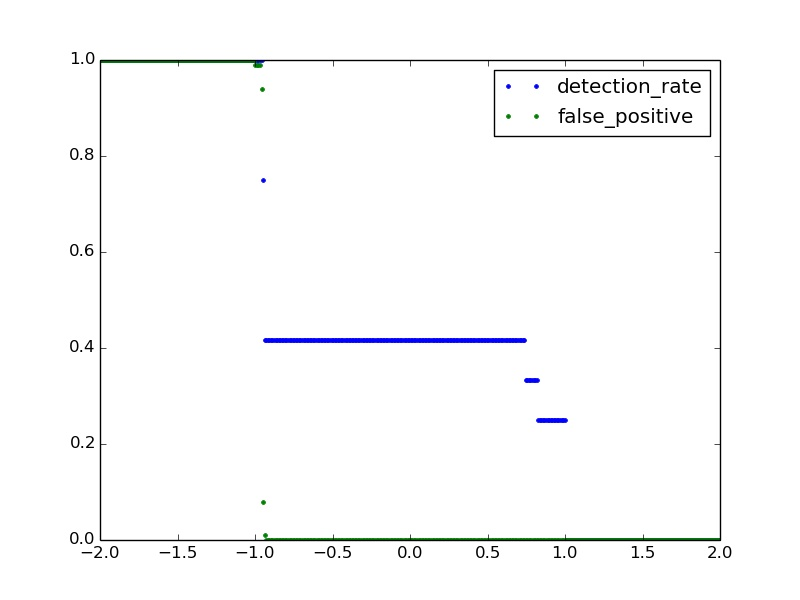
\includegraphics[height=10cm]{./graphics/AdaBoostRegressor_5E0.1L.jpg}

图1. 

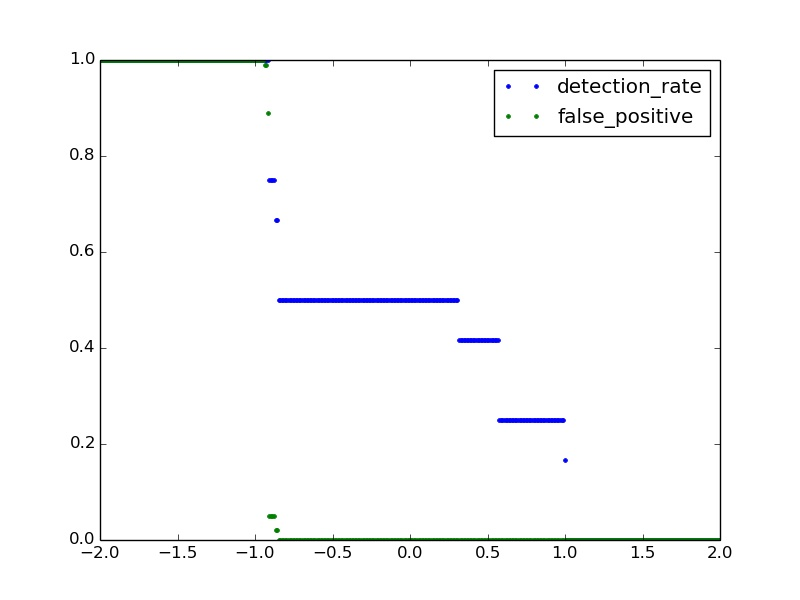
\includegraphics[height=10cm]{./graphics/AdaBoostRegressor_6E0.5L.jpg}

图2.

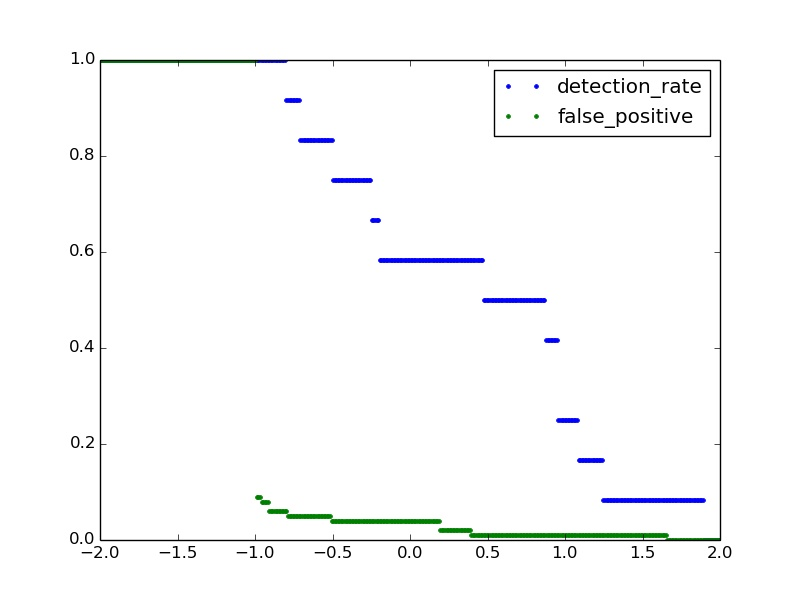
\includegraphics[height=10cm]{./graphics/GradientBoostingRegressor_4E0.6L.jpg}

图3.

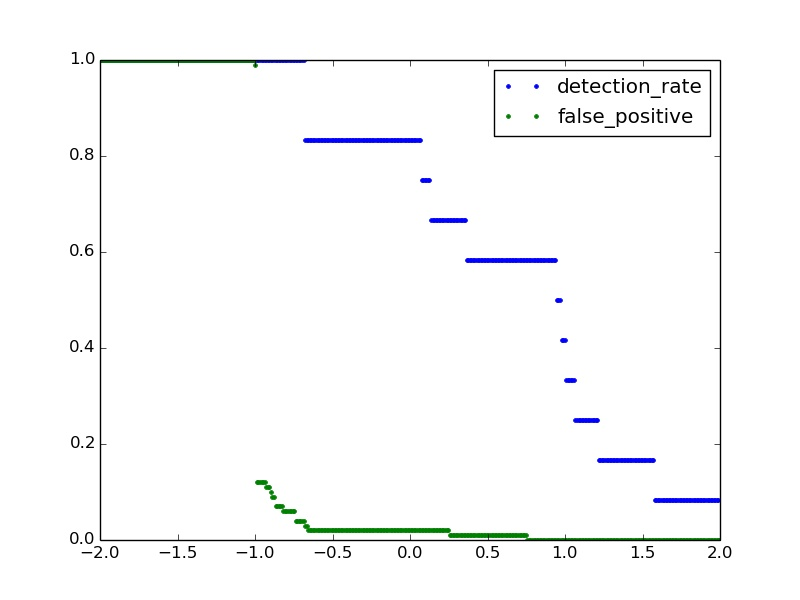
\includegraphics[height=10cm]{./graphics/GradientBoostingRegressor_6E0.5L.jpg}

图4. 

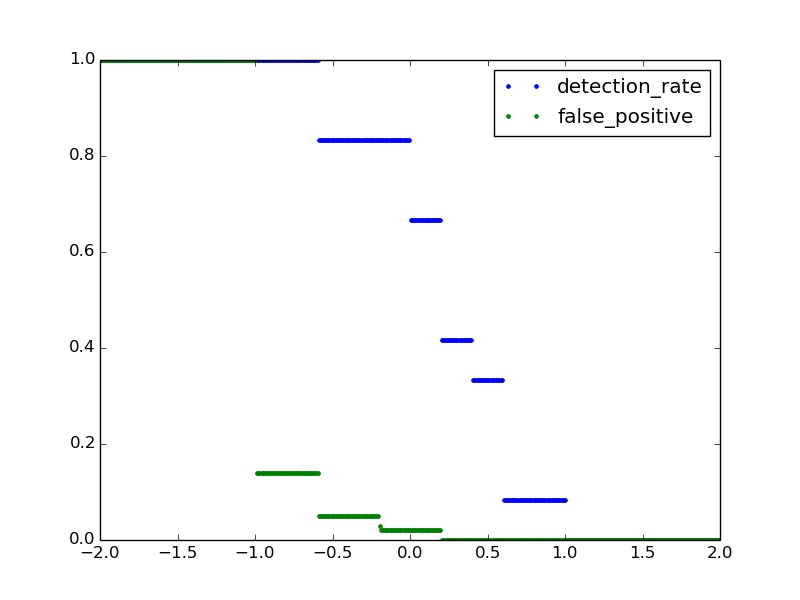
\includegraphics[height=10cm]{./graphics/RandomForestRegressor_5E.jpg}

图5. 

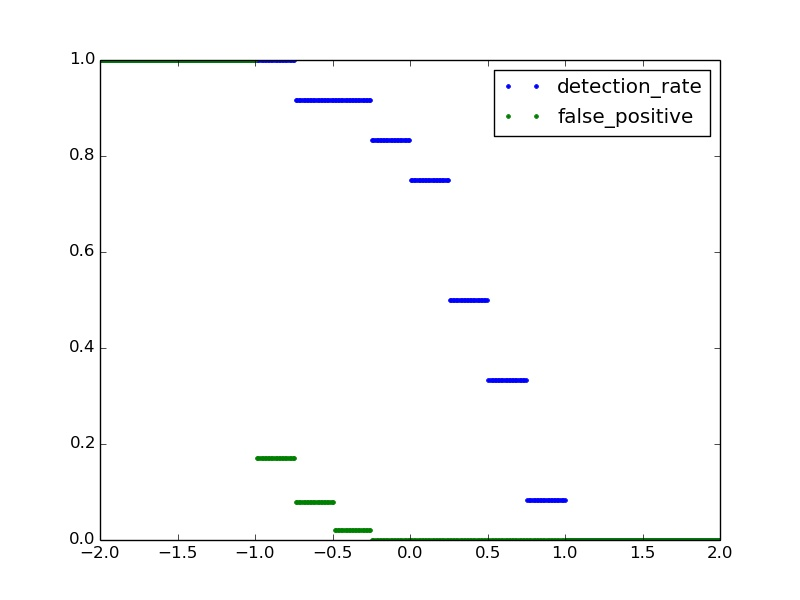
\includegraphics[height=10cm]{./graphics/RandomForestRegressor_8E.jpg}

图6.

\end{center}

\end{document}
